\subsection{Оптимизация визуального интерфейса программы}

Ввиду того, что для оптимизации интерфейса приложения было принято решение отказаться от фреймворка Vue, интерфейс приложения разрабатывался с самого начала.

Разработка происходила с использованием библиотеки React. Для подключения React к странице приложения, необходимо создать корневой элемент приложения (с id равным ``root''), к которому с помощью тега ``script'' будет подключаться библиотека и сгенерированное React-приложение. Подключение представлено на рисунке~\ref{img:reactHTML}

\begin{figure}[H]
  \centering
  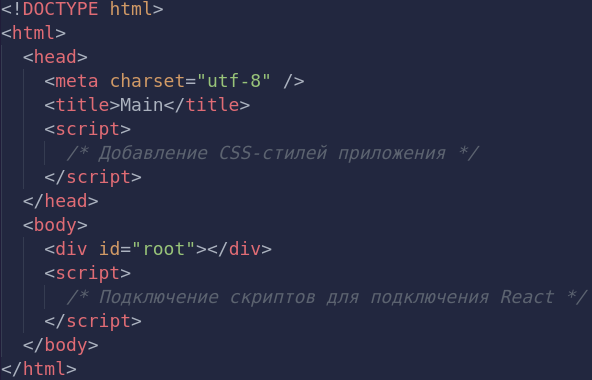
\includegraphics[height=0.2\textheight]{assets/images/practical/reactHTML.png}
  \caption{Подключение React к HTML}
  \label{img:reactHTML}
\end{figure}

Для проверки орфографии была переопределёна стандартная функция, предоставляемая Electron, доступ к которой был получен при расширении контекста процесса. Новый обработчик представлен на рисунке~\ref{img:spellCheckProvider}.

\begin{figure}[H]
  \centering
  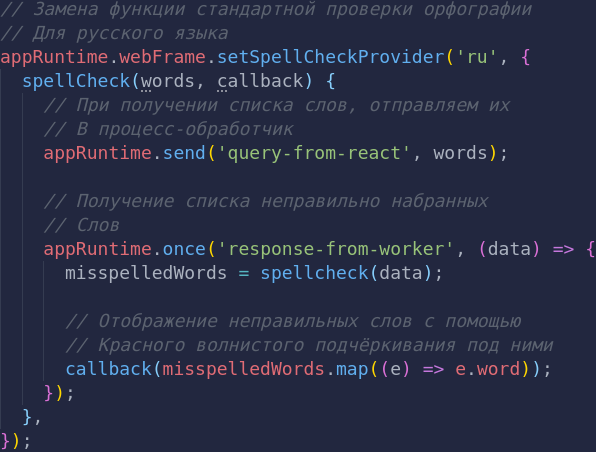
\includegraphics[height=0.2\textheight]{assets/images/practical/spellCheckProvider.png}
  \caption{Подключение React к HTML}
  \label{img:spellCheckProvider}
\end{figure}

Полный код разработанного React-приложения приведен в листингах~\ref{lst:reacMain} и \ref{lst:reactSub}.